% Options for packages loaded elsewhere
\PassOptionsToPackage{unicode}{hyperref}
\PassOptionsToPackage{hyphens}{url}
%
\documentclass[
]{article}
\usepackage{lmodern}
\usepackage{amssymb,amsmath}
\usepackage{ifxetex,ifluatex}
\ifnum 0\ifxetex 1\fi\ifluatex 1\fi=0 % if pdftex
  \usepackage[T1]{fontenc}
  \usepackage[utf8]{inputenc}
  \usepackage{textcomp} % provide euro and other symbols
\else % if luatex or xetex
  \usepackage{unicode-math}
  \defaultfontfeatures{Scale=MatchLowercase}
  \defaultfontfeatures[\rmfamily]{Ligatures=TeX,Scale=1}
\fi
% Use upquote if available, for straight quotes in verbatim environments
\IfFileExists{upquote.sty}{\usepackage{upquote}}{}
\IfFileExists{microtype.sty}{% use microtype if available
  \usepackage[]{microtype}
  \UseMicrotypeSet[protrusion]{basicmath} % disable protrusion for tt fonts
}{}
\makeatletter
\@ifundefined{KOMAClassName}{% if non-KOMA class
  \IfFileExists{parskip.sty}{%
    \usepackage{parskip}
  }{% else
    \setlength{\parindent}{0pt}
    \setlength{\parskip}{6pt plus 2pt minus 1pt}}
}{% if KOMA class
  \KOMAoptions{parskip=half}}
\makeatother
\usepackage{xcolor}
\IfFileExists{xurl.sty}{\usepackage{xurl}}{} % add URL line breaks if available
\IfFileExists{bookmark.sty}{\usepackage{bookmark}}{\usepackage{hyperref}}
\hypersetup{
  pdftitle={Final Report - Kallikrein genes},
  hidelinks,
  pdfcreator={LaTeX via pandoc}}
\urlstyle{same} % disable monospaced font for URLs
\usepackage[margin=1in]{geometry}
\usepackage{color}
\usepackage{fancyvrb}
\newcommand{\VerbBar}{|}
\newcommand{\VERB}{\Verb[commandchars=\\\{\}]}
\DefineVerbatimEnvironment{Highlighting}{Verbatim}{commandchars=\\\{\}}
% Add ',fontsize=\small' for more characters per line
\usepackage{framed}
\definecolor{shadecolor}{RGB}{248,248,248}
\newenvironment{Shaded}{\begin{snugshade}}{\end{snugshade}}
\newcommand{\AlertTok}[1]{\textcolor[rgb]{0.94,0.16,0.16}{#1}}
\newcommand{\AnnotationTok}[1]{\textcolor[rgb]{0.56,0.35,0.01}{\textbf{\textit{#1}}}}
\newcommand{\AttributeTok}[1]{\textcolor[rgb]{0.77,0.63,0.00}{#1}}
\newcommand{\BaseNTok}[1]{\textcolor[rgb]{0.00,0.00,0.81}{#1}}
\newcommand{\BuiltInTok}[1]{#1}
\newcommand{\CharTok}[1]{\textcolor[rgb]{0.31,0.60,0.02}{#1}}
\newcommand{\CommentTok}[1]{\textcolor[rgb]{0.56,0.35,0.01}{\textit{#1}}}
\newcommand{\CommentVarTok}[1]{\textcolor[rgb]{0.56,0.35,0.01}{\textbf{\textit{#1}}}}
\newcommand{\ConstantTok}[1]{\textcolor[rgb]{0.00,0.00,0.00}{#1}}
\newcommand{\ControlFlowTok}[1]{\textcolor[rgb]{0.13,0.29,0.53}{\textbf{#1}}}
\newcommand{\DataTypeTok}[1]{\textcolor[rgb]{0.13,0.29,0.53}{#1}}
\newcommand{\DecValTok}[1]{\textcolor[rgb]{0.00,0.00,0.81}{#1}}
\newcommand{\DocumentationTok}[1]{\textcolor[rgb]{0.56,0.35,0.01}{\textbf{\textit{#1}}}}
\newcommand{\ErrorTok}[1]{\textcolor[rgb]{0.64,0.00,0.00}{\textbf{#1}}}
\newcommand{\ExtensionTok}[1]{#1}
\newcommand{\FloatTok}[1]{\textcolor[rgb]{0.00,0.00,0.81}{#1}}
\newcommand{\FunctionTok}[1]{\textcolor[rgb]{0.00,0.00,0.00}{#1}}
\newcommand{\ImportTok}[1]{#1}
\newcommand{\InformationTok}[1]{\textcolor[rgb]{0.56,0.35,0.01}{\textbf{\textit{#1}}}}
\newcommand{\KeywordTok}[1]{\textcolor[rgb]{0.13,0.29,0.53}{\textbf{#1}}}
\newcommand{\NormalTok}[1]{#1}
\newcommand{\OperatorTok}[1]{\textcolor[rgb]{0.81,0.36,0.00}{\textbf{#1}}}
\newcommand{\OtherTok}[1]{\textcolor[rgb]{0.56,0.35,0.01}{#1}}
\newcommand{\PreprocessorTok}[1]{\textcolor[rgb]{0.56,0.35,0.01}{\textit{#1}}}
\newcommand{\RegionMarkerTok}[1]{#1}
\newcommand{\SpecialCharTok}[1]{\textcolor[rgb]{0.00,0.00,0.00}{#1}}
\newcommand{\SpecialStringTok}[1]{\textcolor[rgb]{0.31,0.60,0.02}{#1}}
\newcommand{\StringTok}[1]{\textcolor[rgb]{0.31,0.60,0.02}{#1}}
\newcommand{\VariableTok}[1]{\textcolor[rgb]{0.00,0.00,0.00}{#1}}
\newcommand{\VerbatimStringTok}[1]{\textcolor[rgb]{0.31,0.60,0.02}{#1}}
\newcommand{\WarningTok}[1]{\textcolor[rgb]{0.56,0.35,0.01}{\textbf{\textit{#1}}}}
\usepackage{graphicx,grffile}
\makeatletter
\def\maxwidth{\ifdim\Gin@nat@width>\linewidth\linewidth\else\Gin@nat@width\fi}
\def\maxheight{\ifdim\Gin@nat@height>\textheight\textheight\else\Gin@nat@height\fi}
\makeatother
% Scale images if necessary, so that they will not overflow the page
% margins by default, and it is still possible to overwrite the defaults
% using explicit options in \includegraphics[width, height, ...]{}
\setkeys{Gin}{width=\maxwidth,height=\maxheight,keepaspectratio}
% Set default figure placement to htbp
\makeatletter
\def\fps@figure{htbp}
\makeatother
\setlength{\emergencystretch}{3em} % prevent overfull lines
\providecommand{\tightlist}{%
  \setlength{\itemsep}{0pt}\setlength{\parskip}{0pt}}
\setcounter{secnumdepth}{-\maxdimen} % remove section numbering
\usepackage{float}

\title{Final Report - Kallikrein genes}
\author{}
\date{\vspace{-2.5em}19.07.2021}

\begin{document}
\maketitle

\thispagestyle{empty}
\hrule
\vspace{0.3cm}
\begin{center}
    \vspace{1cm}
  \large
    \begin{tabular}[c]{l}
     \\

Anouk Dupe, David Eckey, Dustin Schilling, Maria Yemane \\
\\
     \\
    Supervisor:
    Dr. Maria Dinkelacker \\
     \\
    Tutor:
    Nils Mechtel \\
     \\
     \\
    Data Analysis for students of Molecular Biotechnology \\
    \\
    Heidelberg University 
    \vspace{0.3cm} \\
    \end{tabular}
    \end{center}

\begin{center}\rule{0.5\linewidth}{0.5pt}\end{center}

\pagenumbering{gobble}
\pagebreak
\tableofcontents
\pagebreak
\pagenumbering{arabic}

\hypertarget{introduction}{%
\subsection{1. Introduction}\label{introduction}}

KLKs are a family of 15 mammalian secreted serine proteases. Analysis
has shown that the KLK locus is most likely located on chromosome 19 and
forms the largest cluster of contiguous proteases in the entire genome.
(Yousef et al.~2000).\\
All 15 kallikrein genes are proteolytic enzymes of steroid hormone
regulation and are involved in the regulation of blood pressure, tissue
remodeling, skin desquamation, and many other processes. The structure
of KLK are similar with two beta-drums, two alpha-helices and a distinct
loop involved in the regulation of activity and selectivity. Currently,
the specific role of each kallikrein is unclear. It is known that they
are involved in the complex regulatory processes, more specifically in
those different signaling cascades.\\
Dysregulation of KLKs are frequently associated with cancer. Their
expression in different tissues and their involvement in different
physiological processes make them potential tumor expression markers
(Fischer and Meyer-Hoffert, 2013).\\
Differential expression of different kallikrein genes has been found in
different cancer types. While clear cell and papillary renal carcinomas
have similar kallikrein expression profiles, chromophobe renal cell
carcinoma has a unique expression profile (Tailor et al.~2018).

In the following, a set of in total 32 microarrays will be analysed. 20
of those originate from patients with breast cancer derived from the
data set GSE65216 (Maire et al.~2013), 12 from patients with small cell
lung cancer from GSE149507 (Cai et al.~2021). In this report, both
cancer types are analyzed seperatively and both their results will be
discussed later on.

\hypertarget{quality-control}{%
\subsection{2. Quality control}\label{quality-control}}

After reading in the data, the first step is to verify its quality by
following the steps presented in ``R Course Micoarray Analysis'' by
Dr.~Maria Dinkelacker (2019). The goal of quality control is to identify
samples for which the data characteristics are significantly different.
These differences would be difficult to remove via variance stabilizing
normalisation (vsn) and could interfere with the rest of the data.
Samples that show odd characteristics will thereby be identified and
replaced in the following quality control. The quality control is
performed on the breast cancer microarray data set GSE65216 (Maire et
al.~2013) and the small cell lung cancer microarray data set GSE149507
(Cai et al.~2021).

\hypertarget{quality-control---gse65216-breast-cancer}{%
\subsubsection{2.1 Quality control - GSE65216 breast
cancer}\label{quality-control---gse65216-breast-cancer}}

Upon examination of each individual array, there are no scratches or
lighter areas detectable, which means the arrays themselves are fine.
Furthermore, the meanSd plot is being used to verify the variance
stabilization. Here, the red line, which stands for the running median,
should be horizontal. However for the breast cancer data, it follows a
linear relationship.

\begin{Shaded}
\begin{Highlighting}[]
\NormalTok{knitr}\OperatorTok{::}\KeywordTok{include_graphics}\NormalTok{(}\StringTok{"images/breast_meansdPlot.png"}\NormalTok{)}
\end{Highlighting}
\end{Shaded}

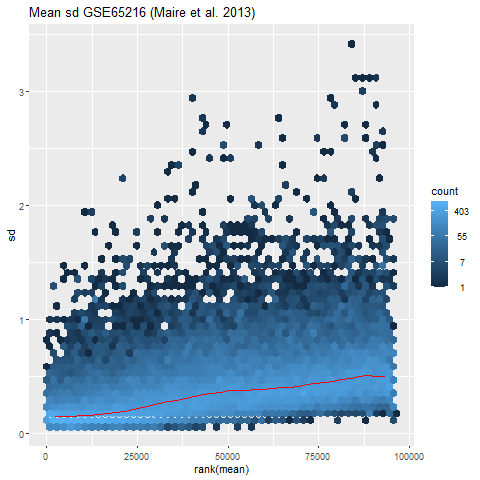
\includegraphics[width=0.3\linewidth,style="float:right; padding:10px"]{images/breast_meansdPlot}

In contrast to that, the quality of the breast cancer data is assured by
the other plots, which is the reason why our group did not choose other
chips for the data analysis. For the boxplots, it is clearly visible,
that the differences in intensities between arrays is strongly reduced
after normalisation. The boxplots only show little fluctuation in gene
expression for the 20 arrays after normalisation. In addition to that,
none of the current chips deviate strongly from each other for the
density and RNA degradation plot (before and after normalisation). Also,
the scatter plots show linear relationships between each chip. The
quality control plots can be seen in the github repository.

\hypertarget{quality-control---gse149507-lung-cancer}{%
\subsubsection{2.2 Quality control - GSE149507 lung
cancer}\label{quality-control---gse149507-lung-cancer}}

For the small cell lung cancer microarray, an abnormality was dectable
in the scatter plots. The carcinoma tissue sample of patient number 5
did not show linear relationship to all of the other samples. Since the
samples of dataset GSE149507 for normal and carcinoma tissue are linked
to one patient each, we consequently replaced the two chips
GSM4504109\_SCLC\_05\_ca and GSM4504110\_SCLC\_05\_n with new 2 new
chips out of the gene expression omnibus. When performing the scatter
plot control over again, there are no discrepancies.\\

\begin{figure}

{\centering 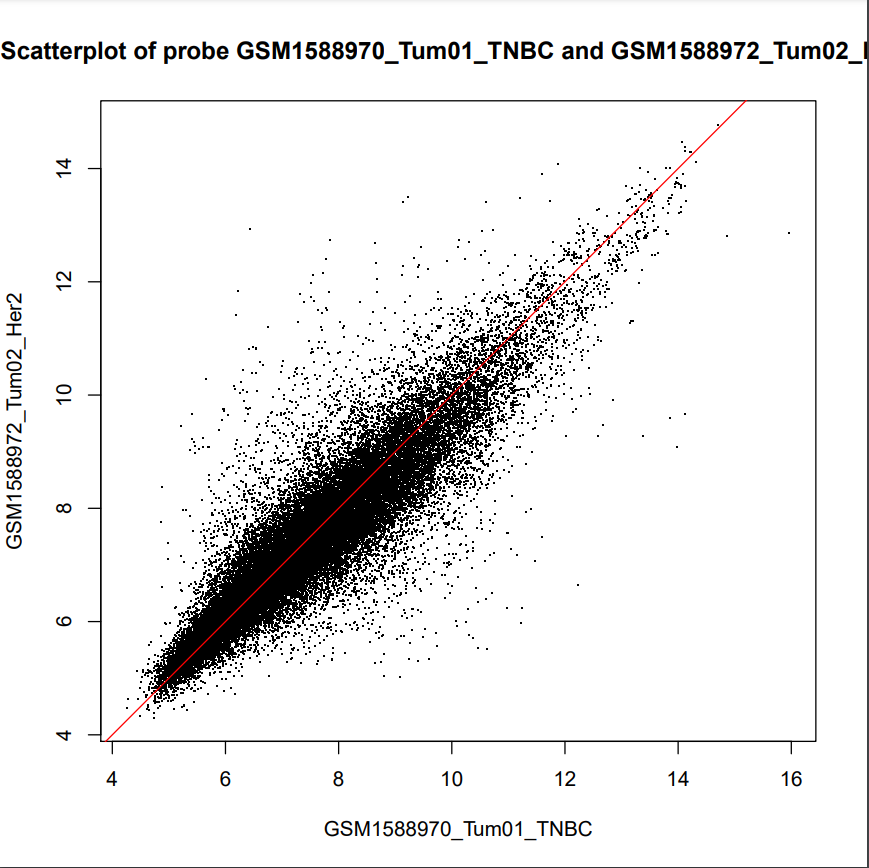
\includegraphics[width=0.5\linewidth]{images/breast_scatter_example1} 

}

\caption{Example of scatter plot breast cancer GSE65216.}\label{fig:Broken chip - lung qc}
\end{figure}

Equivalent to the breast cancer microarray, there were no further
abnormalities detectable for the lung cancer microarray.

\hypertarget{tra-data}{%
\subsection{3. TRA data}\label{tra-data}}

\begin{figure}

{\centering 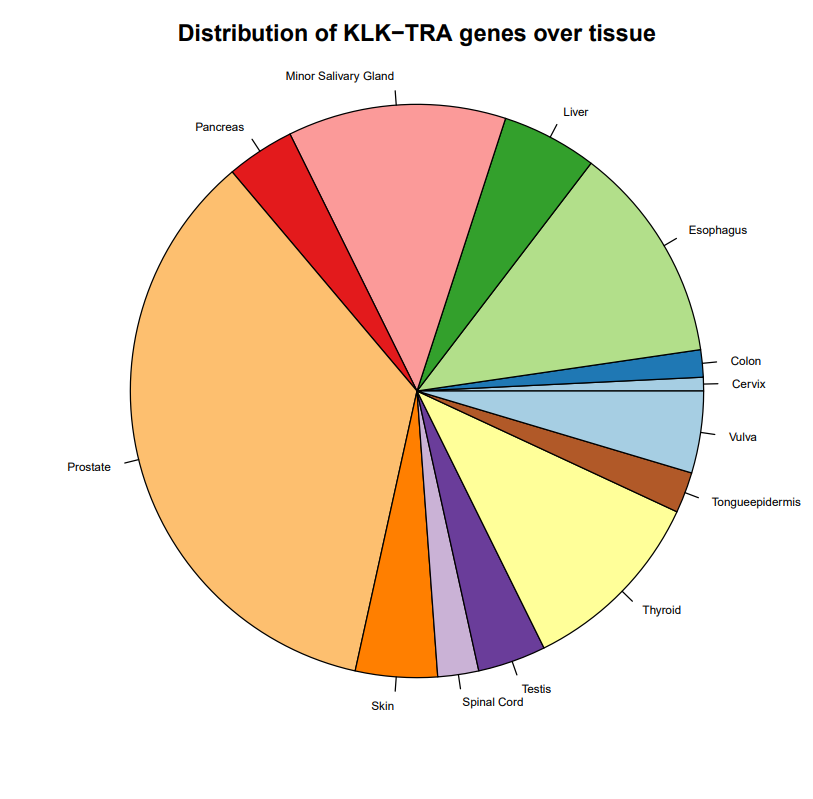
\includegraphics[width=0.5\linewidth]{images/piechart_TRA} 

}

\caption{Tissue specificy of KLK genes - KLK genes from six TRA datasets are combined and sorted for tissue specificity}\label{fig:TRA -piechart}
\end{figure}

To distinguish between TRA KLK genes and non-TRA KLK genes, a total of 6
TRA data sets were utilized ((Su et al.~2002, 2004), (Roth et al.~2008),
(Lattin et al.~2006), (human GTEX data 2015), (Uhlén et al.~2015)).
These TRA data sets were than unified, which allowed the extraction of
tissue-restricted KLKs after their transcription number.\\
To get an overview of the distribution of the Tissue Restricted
Antigens, especially those that are Kallikrein genes, a pie chart was
conducted. A pie chart in general allows a quick overview and a first
assessment of numerical distribution values. In this pie chart, the
distribution of Tissue Restricted Kallikrein-Antigens is displayed.
Notable is the high prevalence of prostatic kallikrein genes, as well as
an occurrence in esophagus, thyroid and salivary gland. Since six data
sets were combined, annotations for the same tissue were different,
which were fused manually.

\hypertarget{expression-analysis}{%
\subsection{4. Expression Analysis}\label{expression-analysis}}

\hypertarget{breast-cancer-gse65216-maire-et-al.-2013}{%
\subsection{4.1 Breast cancer GSE65216 (Maire et
al.~2013)}\label{breast-cancer-gse65216-maire-et-al.-2013}}

The breast cancer microarray data GSE65216 (Maire et al.~2013) consists
of 20 samples. The samples are all breast cancer tissue, differentiated
by the four mutation types: Triple negative breast cancer (TNBC), Her2,
Luminal A and Luminal B.

\hypertarget{clean-up-identical-isoforms}{%
\subsubsection{Clean up identical
isoforms}\label{clean-up-identical-isoforms}}

Having a look onto the data set itself, it is noticeable, that some of
the expression values of the KLK isoforms in the microarray are exactly
identical. These identical isoforms should be cleared out to increase
the real information value of the KLKs. This is easily done by
conducting pairwise correlations, here the pearson correlation, between
all KLK genes in a diagonal matrix. If the correlation yields a value of
1 then the two gene isoforms are the same and the latter one of both
will be removed. Furthermore, the KLKs are sorted after their names in
ascending order for the later visualization. In the end, 39 identical
isoforms are removed, whereas a total of 73 KLK transcripts for the 15
KLK genes are being kept. Out of the 73 isoforms, 63 are TRAs, while
only 10 are regarded as tissue restricted.

\begin{Shaded}
\begin{Highlighting}[]
\CommentTok{# transform dataset - genes on columns}
\NormalTok{df.TRA.KLK.breast <-}\StringTok{ }\KeywordTok{data.frame}\NormalTok{(}\KeywordTok{t}\NormalTok{(TRA.KLK.breast))}

\CommentTok{# Define function for calculating correlation }
\NormalTok{cor.genes <-}\StringTok{ }\ControlFlowTok{function}\NormalTok{(df)\{}
\NormalTok{  df.cor <-}\StringTok{ }\KeywordTok{cor}\NormalTok{(df, }\DataTypeTok{method =} \StringTok{"pearson"}\NormalTok{)}
  \KeywordTok{diag}\NormalTok{(df.cor)=}\OtherTok{NA}
\NormalTok{  df.cor[}\KeywordTok{upper.tri}\NormalTok{(df.cor)]=}\OtherTok{NA}
  \KeywordTok{return}\NormalTok{(}\KeywordTok{data.frame}\NormalTok{(df.cor))}
\NormalTok{\}}

\CommentTok{# amount of identical columns}
\NormalTok{cor.TRA.KLK.breast <-}\StringTok{ }\KeywordTok{cor.genes}\NormalTok{(df.TRA.KLK.breast)}
\KeywordTok{length}\NormalTok{(}\KeywordTok{which}\NormalTok{(cor.TRA.KLK.breast }\OperatorTok{==}\StringTok{ }\DecValTok{1}\NormalTok{))}
\end{Highlighting}
\end{Shaded}

\begin{verbatim}
## [1] 35
\end{verbatim}

\begin{Shaded}
\begin{Highlighting}[]
\CommentTok{# cleanup function }
\NormalTok{genes.cleanup <-}\StringTok{ }\ControlFlowTok{function}\NormalTok{(df)\{}
\NormalTok{  df[}\OperatorTok{!}\KeywordTok{duplicated}\NormalTok{(}\KeywordTok{unclass}\NormalTok{(df))]}
\NormalTok{\}}

\CommentTok{# remove identical columns}
\NormalTok{TRA.KLK.breast.clean <-}\StringTok{ }\KeywordTok{genes.cleanup}\NormalTok{(df.TRA.KLK.breast)}
\KeywordTok{dim}\NormalTok{(TRA.KLK.breast.clean)}
\end{Highlighting}
\end{Shaded}

\begin{verbatim}
## [1] 20 63
\end{verbatim}

\hypertarget{overview-gene-expression}{%
\subsubsection{Overview gene
expression}\label{overview-gene-expression}}

Since the data is vsnrma normalized, the median does not fluctuate too
much for all samples. The lowest gene expression value of the first chip
is roughly 6 while the highest gene expression value is around 16. Due
to the logarithmic scale with a base of 2, gene expression is double as
high between two samples if the log-fold change is +1.

\begin{Shaded}
\begin{Highlighting}[]
\NormalTok{gene.summary <-}\StringTok{ }\ControlFlowTok{function}\NormalTok{(x)\{}
 \KeywordTok{round}\NormalTok{(}\KeywordTok{apply}\NormalTok{(x, }\DecValTok{2}\NormalTok{, summary), }\DataTypeTok{digits =} \DecValTok{2}\NormalTok{)}
\NormalTok{\}}
\KeywordTok{gene.summary}\NormalTok{(breastExprs)[,}\DecValTok{1}\NormalTok{]}
\end{Highlighting}
\end{Shaded}

\begin{verbatim}
##    Min. 1st Qu.  Median    Mean 3rd Qu.    Max. 
##    5.57    6.76    7.50    7.81    8.54   15.94
\end{verbatim}

The histogram represent the frequency of the present gene expression in
breast cancer samples. It also shows, that the median gene expression of
KLKs is much lower than the overall median gene expression. This means
that most of the KLK gene expression is normally down-regulated in the
perspective of the whole genome. (Yousef et al.~2004)

\begin{figure}

{\centering 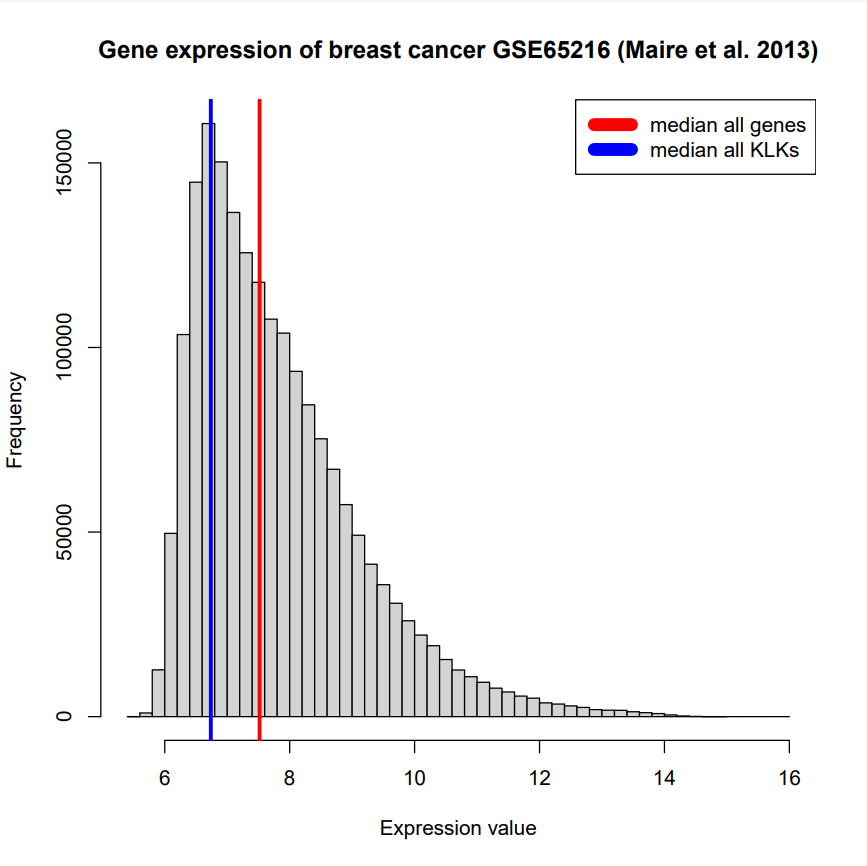
\includegraphics[width=0.5\linewidth]{images/Histogram_breast} 

}

\caption{Histogram of breast cancer gene expression.}\label{fig:Histogram - breast }
\end{figure}

\hypertarget{boxplots}{%
\subsubsection{Boxplots}\label{boxplots}}

\begin{figure}

{\centering 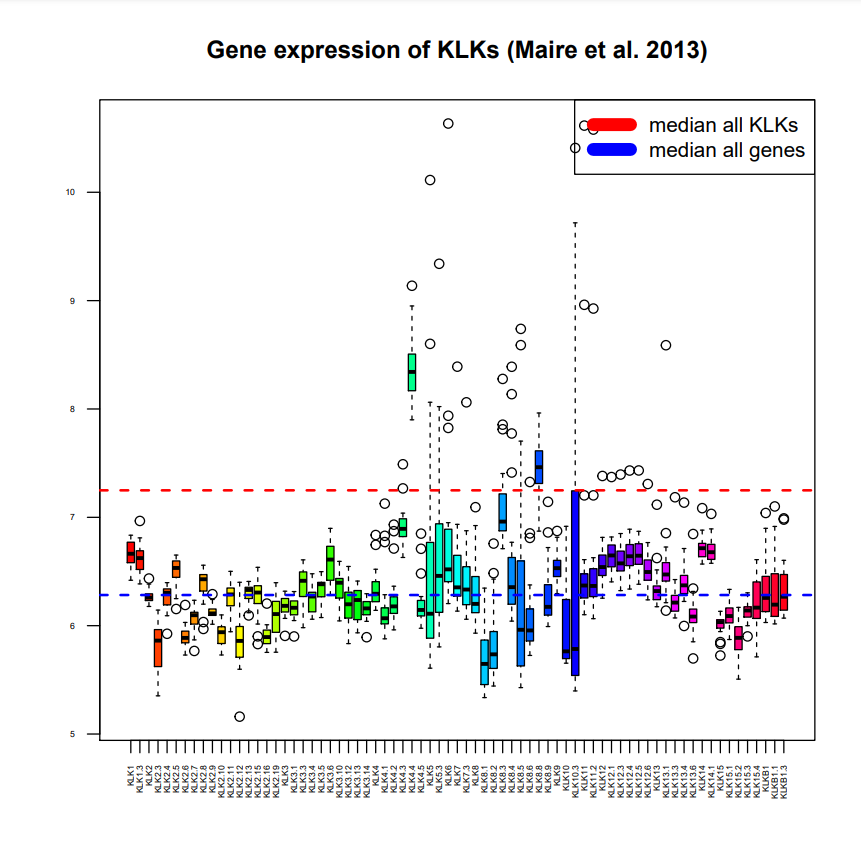
\includegraphics[width=0.5\linewidth]{images/Boxplot_breast} 

}

\caption{Boxplot of KLK gene expression in breast cancer.}\label{fig:Boxplot - breast }
\end{figure}

Here, the pattern for the fairly low gene expression of KLKs is also
recognizable. Most of the boxplots of the single KLK gene isoforms are
lower than the median expression of the whole breast cancer genome. Some
KLK isoforms like KLK2.3 are even below a gene expression value of 6, so
KLK isoforms like these are clearly down-regulated. This is compatible
with the finding of Yousef et al.~in which they state an overall
down-regulation of KLK gene expression in breast cancer. There are only
two isoforms that exceed the median of the whole genome expression of
the breast cancer set. These are the isoforms KLK4.4 and KLK8.8.\\
KLK4 gene expression was found by Schmitt et al.~to be up-regulated in
breast cancer tissue as in comparison to healthy breast tissue. This
seems to correspond with the finding shown in the boxplot, but only for
the KLK4.4 isoform. Thereby, KLK4.4 needs to be looked on more
carefully. In contrast to that, KLK8 seems to be higher expressed in
both normal and cancer tissue.(Schmitt et al.~2013)

\hypertarget{heatmap}{%
\subsubsection{Heatmap}\label{heatmap}}

The dendrogram is the core for the emerging clustering in heatmaps.

\begin{figure}

{\centering 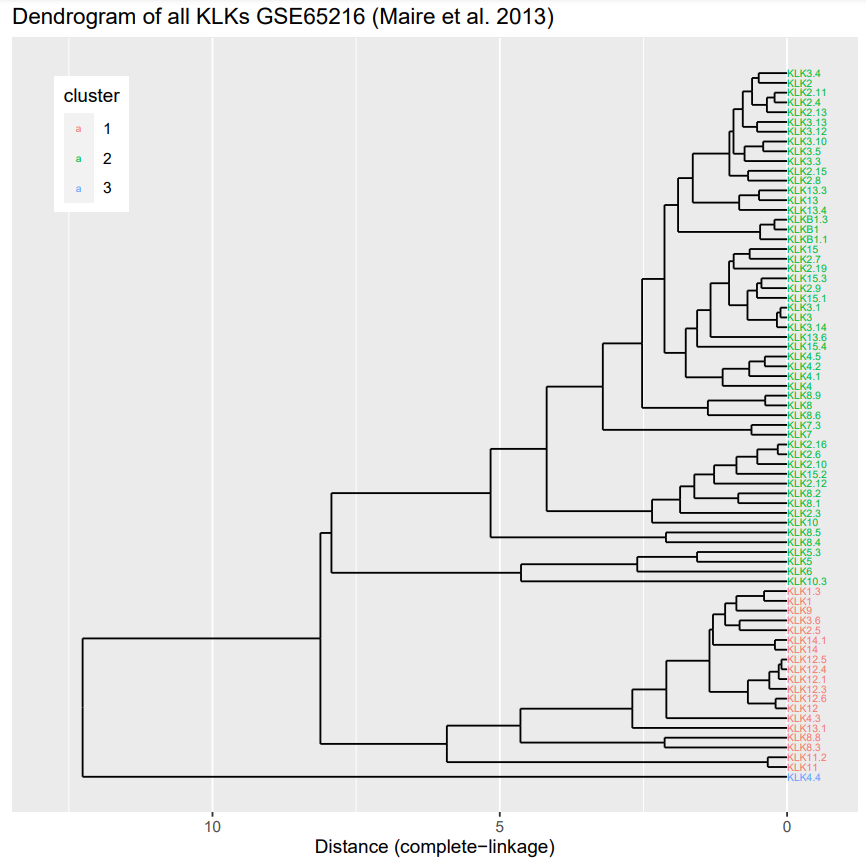
\includegraphics[width=0.5\linewidth]{images/Dendrogram_breast} 

}

\caption{Dendrogram of KLK genes in breast cancer. Clustering is performed after the complete-linkage method. The genes are separated into 3 clusters.}\label{fig:Dendrogram - breast }
\end{figure}

Interesting in this respect is, that KLK4.4 forms its own branch
independent of all the others. As already shown in the boxplots, KLK4.4
was distinctly up-regulated. Looking onto the other branches of the
dendrogram, it is notable that besides KLK4.4 there are more possible
clusters. To increase the clarity of the heatmap, KLKs are separated
into 3 clusters. Optimal clustering via K-means will still be performed
later on.\\

\begin{figure}

{\centering 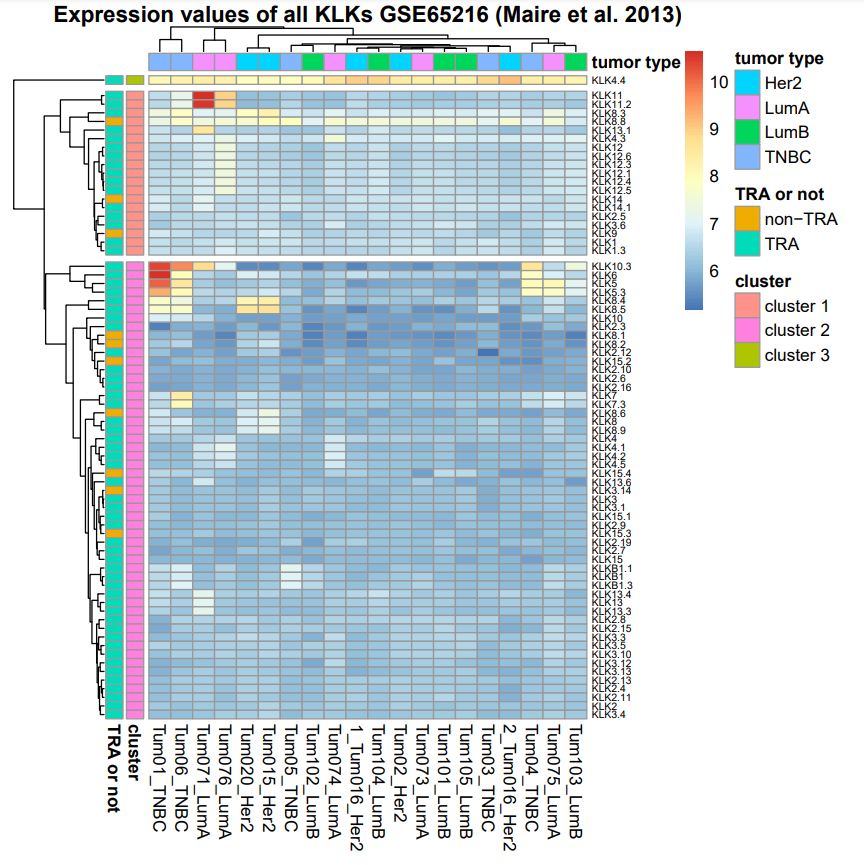
\includegraphics[width=0.5\linewidth]{images/Heatmap_breast} 

}

\caption{Heatmap of KLK gene expression in breast cancer. The samples are annotated corresponding to their mutation type. Additionally, the KLKs are differentiated by their cluster and potential tissue restriction.}\label{fig:Heatmap - breast }
\end{figure}

KLK4.4 clearly stands out (cluster 2) with an overall up-regulated gene
expression across all sample. Furthermore, as it is annotated KLK4.4
belongs to the TRA group. Moreover, gene expression in cluster 1 is
higher than in the third cluster. There are only few samples which seem
to have up-regulated KLK isoforms. For instance, the tumor sample number
1 and 6 (Tum01\_TNBC and Tum01´6\_TNBC) got one of the highest
expression values across all the KLKs for KLK10.3, KLK6 and KLK5. As
well as the tumor sample number 71 and 76 (Tum71\_LumA, Tum76\_LumA) for
the transcripts KLK11 and KLK11.2.

\hypertarget{pca}{%
\subsubsection{PCA}\label{pca}}

The principal component analysis was conducted over the samples.
Centering was enabled, while scaling was not included, due to the data
being vsnrma normalized. The cumulative variance of the first two
principal components (PCs) yield 72\% of the total variance. Thereby,
these two PCs explain 72\% of the total information value. PC1 and PC2
are sufficient for the analysis. The breast cancer samples are
distributed after their respective loadings of KLK gene expression.\\
\textbackslash begin\{figure\}

\{\centering 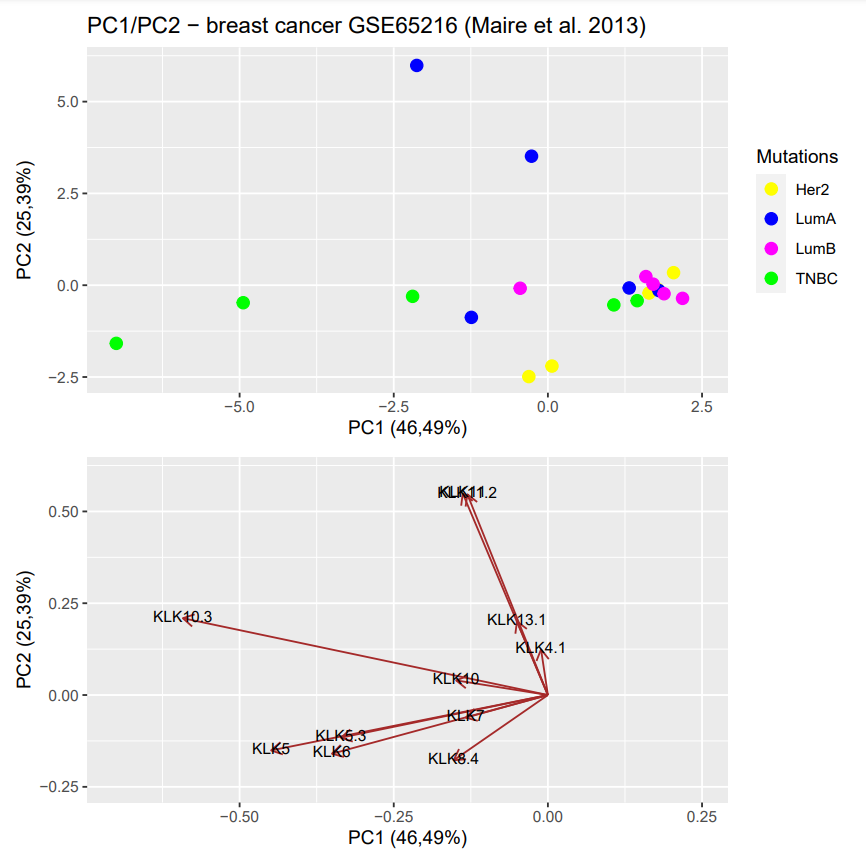
\includegraphics[width=0.5\linewidth]{images/PCAplot_breast}

\}

\textbackslash caption\{PC1 (46,49\%) is plotted against PC2 (25,39\%).
The upper part shows the distribution of the breast cancer samples
annotated by their mutation type, while the lower part depicts the 12
highest loadings of the KLK genes.\}\label{fig:PCA plot - breast }
\textbackslash end\{figure\} The loadings consists of the the top 12
most differentiated KLK isoforms. This was conducted by adding the
absolute values of the rotation matrix for each individual KLK isoform.
As the PCA displays, some samples are more characterized by the
expression of KLK11 and KLK11.2. This is mostly the case for two of the
LumA samples. This was also observable in the heatmap by the higher
expression of KLK11 and KLK11.2 for the tumor samples 71 and 76. Another
finding of the PCA is that TNBC mutations are affected by KLK5 and KLK6
expression, also observable in the heatmap. Presumably KLK4.4 is not
part of the top 12 loadings, since it is higher expressed across all
tumor samples.

\hypertarget{k-means-clustering}{%
\subsubsection{K-means clustering}\label{k-means-clustering}}

K-means was performed to be able to draw conclusions on characteristics
and the distribution of different Kallikrein genes. Here, the optimal
number k of clusters was determined in doing a Within Cluster Sum of
Squares -- plot, also called the elbow method. A kink in the curve of a
plot, in which the number k of clusters is plotted against the within
cluster sum of squares, displays the optimal number of k clusters.
Rising numbers of k will not cause a significant decline in the within
cluster sum of squares anymore. For the breast cancer GSE65216 data set,
the Within Cluster Sum of Squares -- plot predicted an optimal number of
k = 6, so k-means was performed using 6 clusters. The function of
k-means automatically reduces dimensions to 2 if a dataset consists of 3
or more dimensions, so the k-means clustering does not directly cluster
genes of interest according to their expression values, but cluster
according to two dimensions that are influenced by expression values, as
those explain most of the variance of the data. Due to this influence,
k-means is still suited for clustering and thus comparing KLK expression
patterns. Outstanding cluster is here marked as cluster 1 in green,
containing KLKs4.4 and KLK8.8. Those genes already stood out in the
heatmap analysis. Interestingly, cluster 4 is also very distinct but on
the very other direction on the graph of two dimensions.

\begin{figure}

{\centering 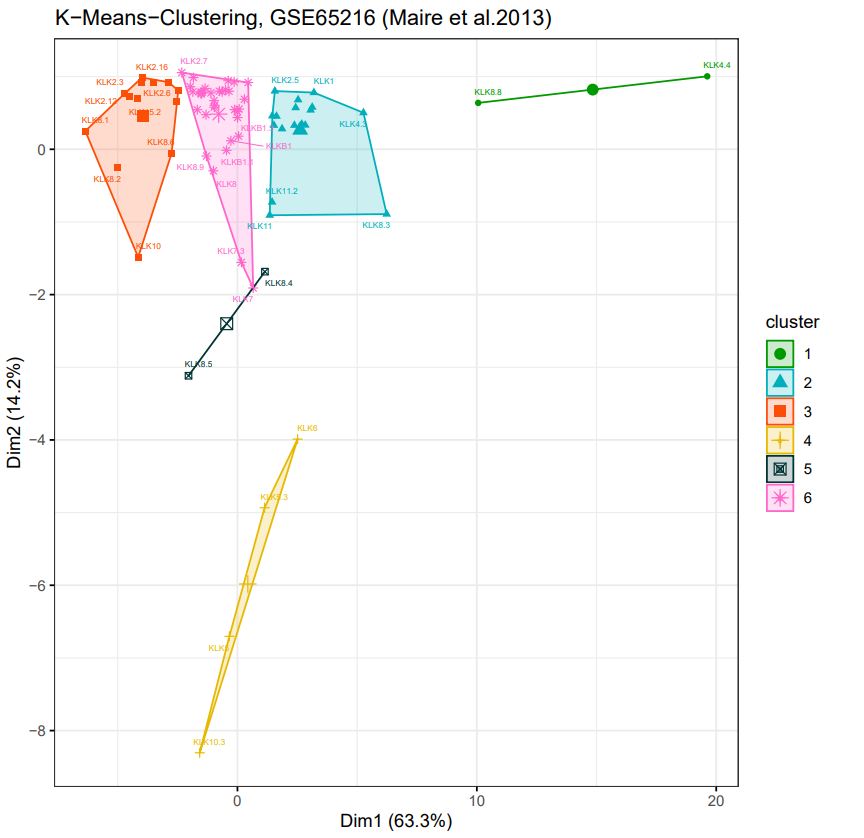
\includegraphics[width=0.5\linewidth]{images/kmeans_6_breast} 

}

\caption{K-means cluster analysis with k = 6 clusters for the breast cancer data set}\label{fig:K-means plot - breast }
\end{figure}

\hypertarget{hypothesis-testing}{%
\subsubsection{Hypothesis testing}\label{hypothesis-testing}}

WILCOX TEST WEITER AUSFÜHREN?! DATENSTRUKTUR ERKLÄREN?!

The expression values of the Kallikrein genes obtained from Marie et
al.~were not normally distributed. Therefore the non- parametric
Wilcoxon-Mann-Whitney-Test was used.

(First, cluster 1 (KLK4.4 and KLK8.8) were tested for overexpression
against all other KLKs individually from the dataset. KLK4.4 (TRA) was
significantly higher expressed than all other KLK genes from the
dataset. Likewise, KLK8.8 (non-TRA) was significantly higher expressed
than all KLK genes, except KLK4.4. Those results conform with the
observations from the heatmap and the k-means clustering. Cluster-4
(KLK5,5.3,6,10.3) was isolated in the k-means clustering. On the heatmap
it was conspicuous that for some tumor types the genes of this cluster
were higher expressed. Thus the upper-tail Wilcoxon-test was used. In
contrast to Cluster-1, Cluster-4 could not be clearly identified as an
overexpression cluster. KLK5.3 and KLK6 were higher expressed than two
thirds of the other KLK genes, wereas KLK5,10.3 were not significantly
higher expressed than most of the other KLKs.)

The main characteristic of the dataset from Marie et al.~is the
subdivision into the samples with different mutations (Her2, LumA, LumB,
TNBC).

\begin{figure}

{\centering 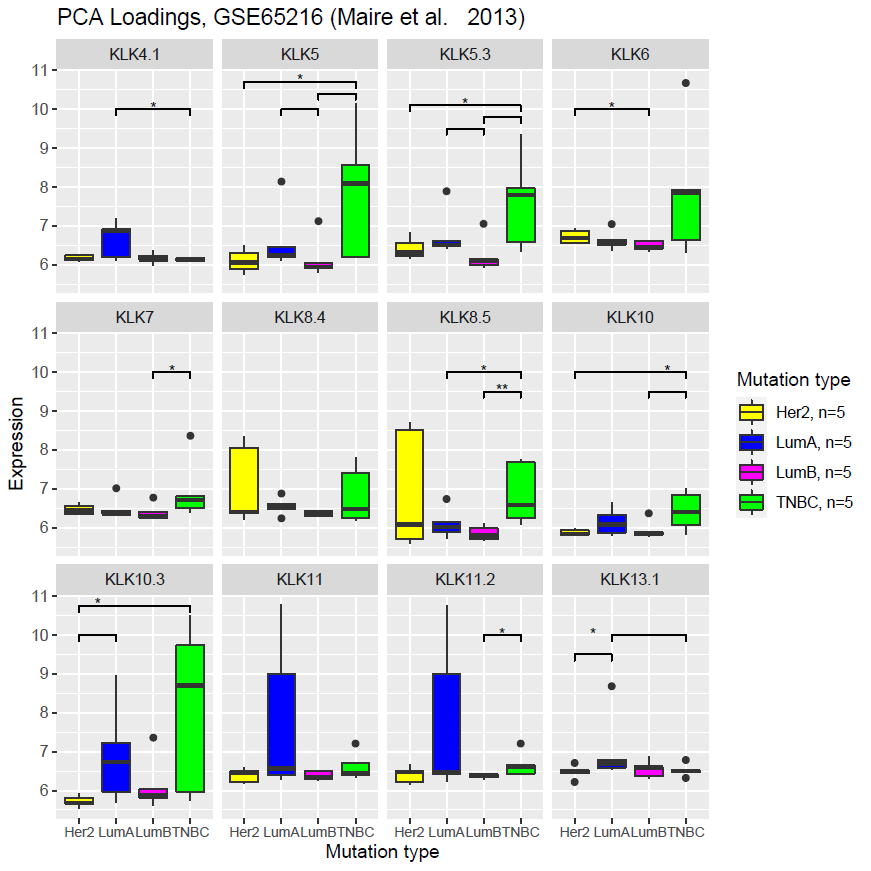
\includegraphics[width=0.5\linewidth]{images/breast_panel_loadings_test} 

}

\caption{Panel plot of the PCA loading genes with significant bars. *: p-value <= 0.5, **: p-value <= 0.01 }\label{fig:Hypothesis test panel plot with significant bars}
\end{figure}

In Figure X, these genes are shown with the subdivision into the
different mutation types. Significant expression differences between
mutation samples are indicated with brackets.

A recurring pattern in Figure X is the significant overexpression of
TNBC compared with Her2. This observation includes KLK5, KLK5.3, KLK10,
KLK10.3.

\hypertarget{lung-cancer-gse149507-cai-et-al.-2021}{%
\subsection{4.2 Lung cancer GSE149507 (Cai et
al.~2021)}\label{lung-cancer-gse149507-cai-et-al.-2021}}

The lung cancer microarray GSE149507 (Cai et al.~2021) derives from six
patients with small cell lung cancer. The data set consists of a total
of 12 samples. Carcinoma tissue and healthy lung tissue, which is
adjacent to the carcinoma, make up 6 samples each.

\hypertarget{overview-gene-expression-1}{%
\subsubsection{Overview gene
expression}\label{overview-gene-expression-1}}

\begin{figure}

{\centering 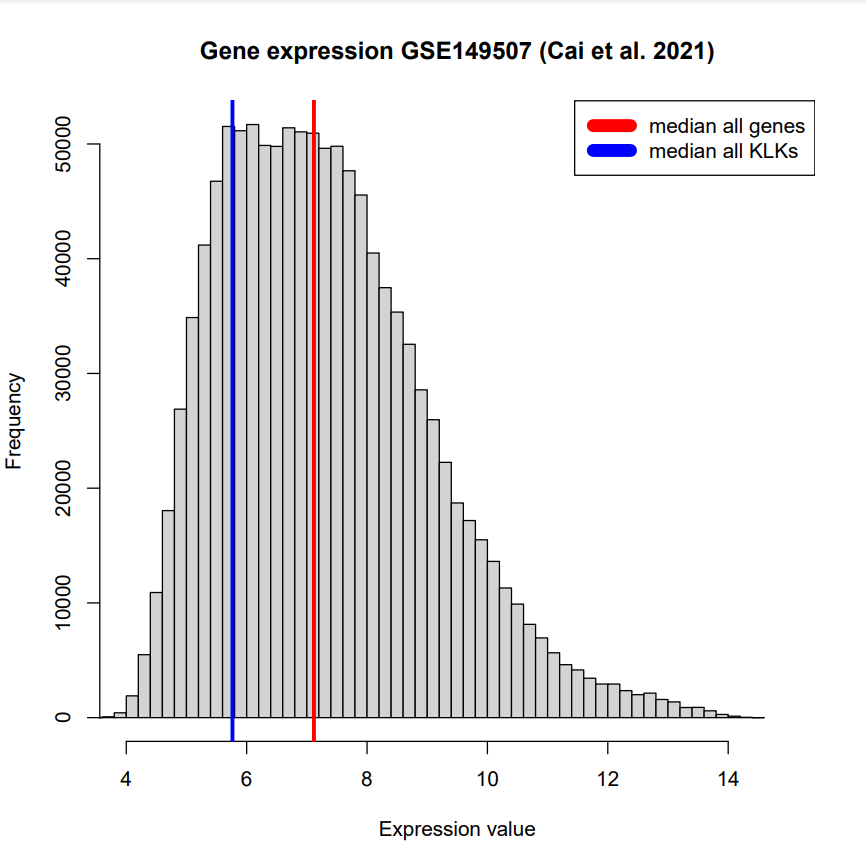
\includegraphics[width=0.5\linewidth]{images/Histogram_lung} 

}

\caption{Histogram of lung cancer gene expression.}\label{fig:Histogram - lung }
\end{figure}

Just as for the breast cancer data set, the median expression of the
KLKs is beneath the the median of the overall gene expression, since
KLKs are mostly down-regulated (Yousef et al.~2004). However for the
lung cancer data set, it appears that the gene expression values are
distributed more evenly, while the breast cancer histogram represents a
right-skewed distribution.

\hypertarget{boxplots-1}{%
\subsubsection{Boxplots}\label{boxplots-1}}

\begin{figure}

{\centering 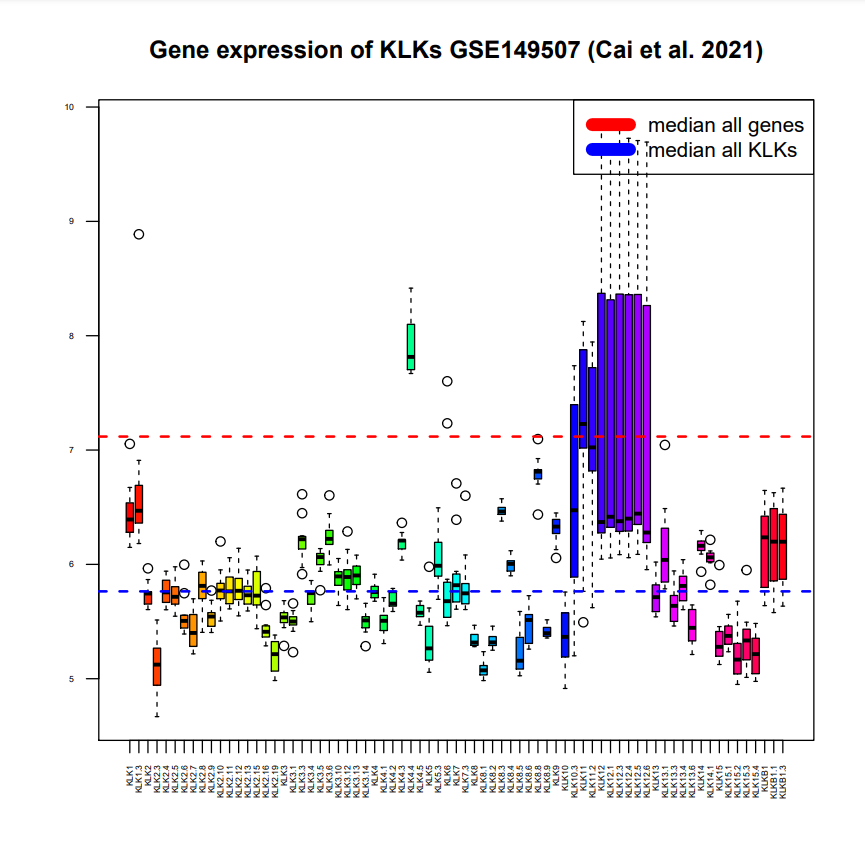
\includegraphics[width=0.5\linewidth]{images/Boxplot_lung} 

}

\caption{Boxplot of KLK gene expression in lung cancer.}\label{fig:Boxplot - lung }
\end{figure}

Most of the KLK boxplots seem to be lower than the overall median gene
expression and thereby are clearly down-regulated. Interestingly, KLK4.4
clearly stands out again as the highest expressed KLK gene. However, it
needs to be considered that the expression of KLK4.4 is around the value
8, which does not really correspond with an over-expression in the
context of the whole genome. Another interesting observation is that the
boxplots of the KLK11 and KLK12 transcripts are big. With the whiskers
of the boxplots, the gene expression spreads from a value of around 6 to
about 9.5. This correlates with a high variety in gene expression for
these gene transcripts. KLK11 and KLK12 gene expression therefore has a
high information value that should be recognizable in the following
methods. This could also be due to the fact that the lung cancer data
set consists of of both normal and healthy tissue, as in comparison to
the breast cancer data set. Here, KLK11 and KLK12 are clear subject for
further investigation in whether they are differently expressed between
normal and carcinoma samples.

\hypertarget{heatmap-1}{%
\subsubsection{Heatmap}\label{heatmap-1}}

\begin{figure}

{\centering 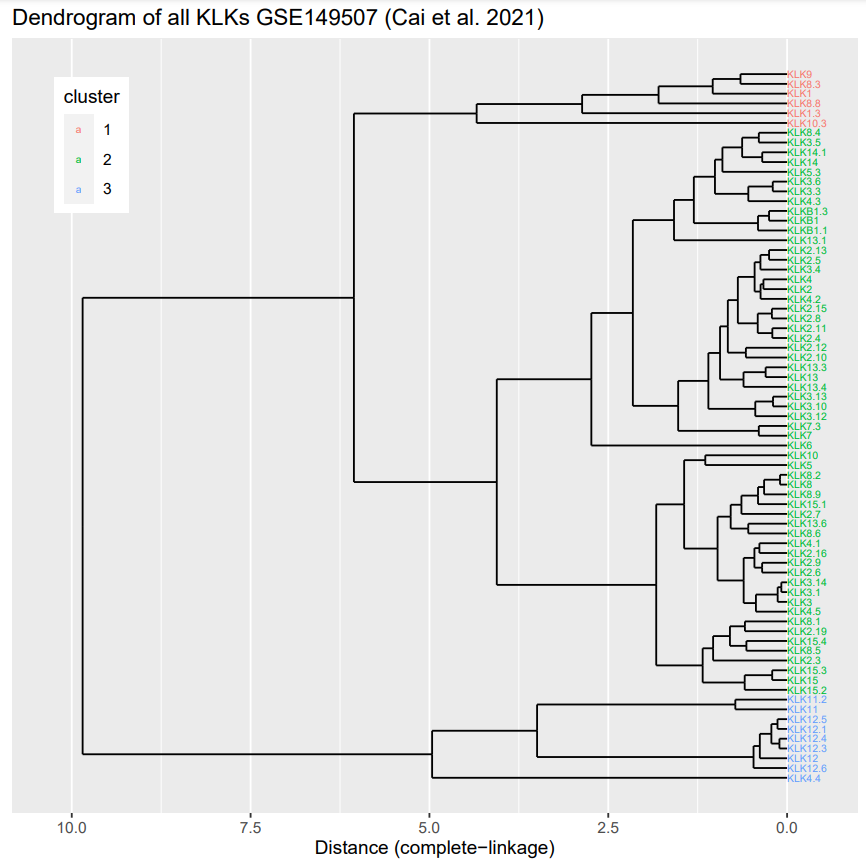
\includegraphics[width=0.5\linewidth]{images/Dendrogram_lung} 

}

\caption{Dendrogram of KLK genes in lung cancer. Clustering is performed after the complete-linkage method. The genes are separated into 3 clusters.}\label{fig:Dendrogram - lung }
\end{figure}

The same strategy as for the breast cancer data set is applied to
improve the quality of the heatmap. The dendrogram shows that multiple
KLK11 and KLK12 isoforms, as well as KLK4.4 are part of one out of the
three clusters.

\begin{figure}

{\centering 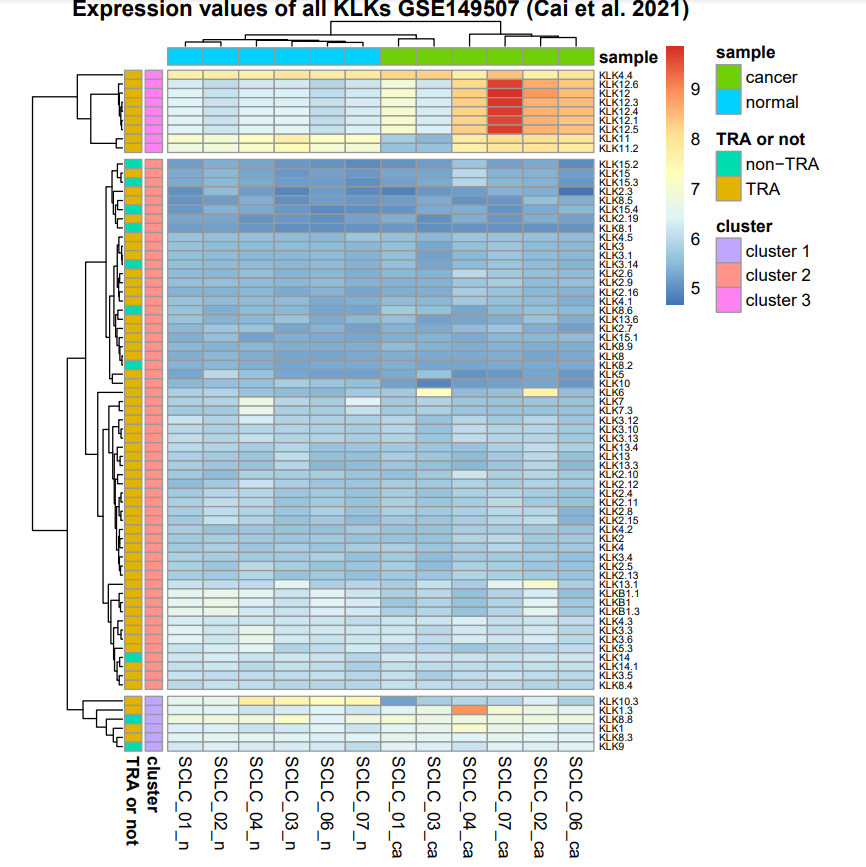
\includegraphics[width=0.5\linewidth]{images/Heatmap_lung} 

}

\caption{Heatmap of KLK gene expression in breast cancer. Carcinoma and normal samples are annotated. Additionally, the KLKs are differentiated by their cluster and potential tissue restriction.}\label{fig:Heatmap - lung }
\end{figure}

Notably, the samples are clustered according to their tissue type being
lung carcinoma or healthy tissue. As you can see in the dendrogram at
the top, the normal samples are clustered into one group with
additionally two more cancer samples. The other four cancer samples all
form their own distinct group. This distribution by sample type clearly
reflects itself in the KLK11 and KLK12 gene expression. While KLK4.4 is
higher expressed for both normal and carcinoma samples, KLK11 and KLK12
isoforms are mainly higher expressed for the carcinoma sample. The only
exception are the already mentioned carcinoma samples SCLC\_01 and
SCLC\_03. Apart from this, the up-regulated gene expression for KLK11
and KLK12 are accompanied by the sample deriving from carcinoma
tissue.\\
As stated by Borgoño et Diamandis, KLK11 up-regulation in lung cancer
was found to have a unfavourable prognosis for the patient. A total of
four out of the six cancer samples have slightly up-regulated KLK11
values. The significance will be tested. The two aforementioned
carcinoma samples SCLC\_01 and SCLC\_03 even got down-regulated KLK11
expression, which thereby might indicate a good chance of treatment
success. (Borgoño et Diamandis 2004)

\hypertarget{pca-1}{%
\subsubsection{PCA}\label{pca-1}}

\textbackslash begin\{figure\}

\{\centering 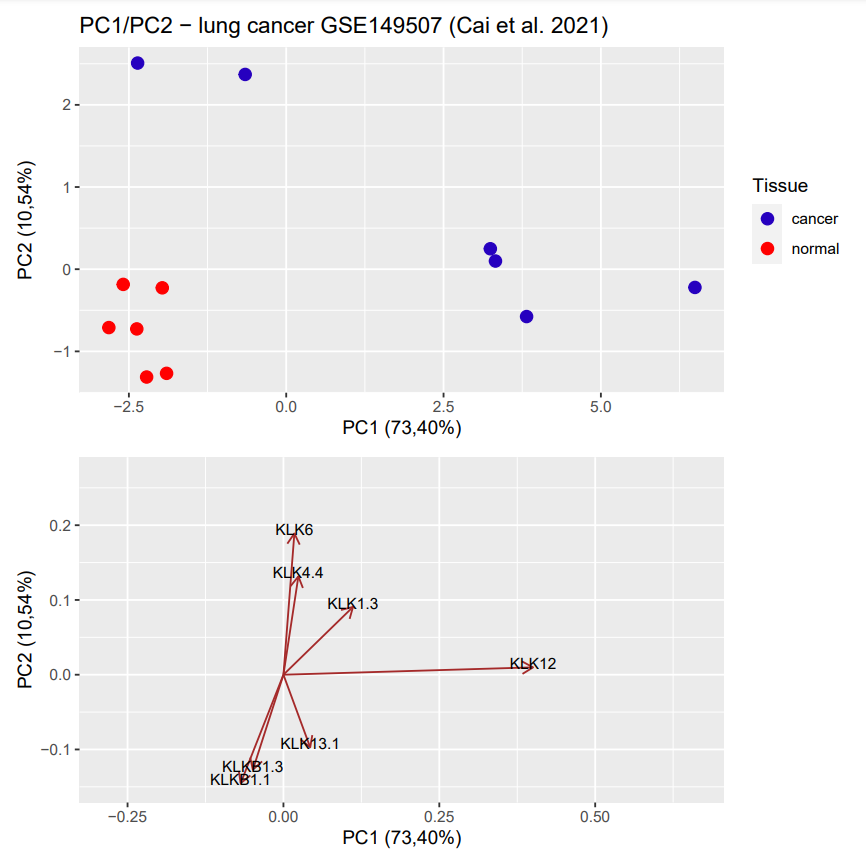
\includegraphics[width=0.5\linewidth]{images/PCAplot_lung}

\}

\textbackslash caption\{PC1 (73,40\%) is plotted against PC2 (10,54\%).
The upper part shows the distribution of the lung cancer samples
annotated by their tissue type, while the lower part depicts the top 7
loadings of the KLKs.\}\label{fig:PCA plot - lung }
\textbackslash end\{figure\} The cumulative variance shows, that 84\% of
the total variance is explained by the first two PCs. These two PCs are
more than sufficient for the analysis. However the first two PCs
covering such a huge proportion of the whole variance corresponds with
an overall low information value of the lung cancer data set.
Considering the heatmap, in which most of expression values were
down-regulated, there is only a low amount of differential gene
expression going on. This explains the high cumulative variance.
Nevertheless, the PCA still shows a clear separation between normal and
carcinoma samples. Considering the loadings, four of the cancer samples
are characterized by KLK12, while the other two tumor samples
SCLC\_01\_ca and SCLC\_03\_ca are mainly represented by KLK4.4 and KLK6
expression. Just as shown in the heatmap, while four out of the six
cancer samples have up-regulated KLK12 expression values, the two cancer
samples SCLC\_01\_ca and SCLC\_03\_ca form an exception. These two do
not go along with the KLK12 loading and are rather defined by KLK6 and
KLK4.4 expression.

\hypertarget{clustering---kmeans}{%
\subsubsection{Clustering - kmeans}\label{clustering---kmeans}}

K-means performed for the lung cancer GSE149507 dataset showed an
interesting and distinct cluster, which only consisted of KLK-subtypes
of KLK12. Other genes that stood out in the heatmap analysis, for
example KLK4.4 and KLK8.8, were found in the first cluster on the top
left corner. The finding of optimal k clusters happened following the
same procedure as for the breast cancer data set, described above. An
optimal number of k = 5 clusters was determined using a Within Cluster
Sum of Squares -- plot.

\begin{figure}

{\centering 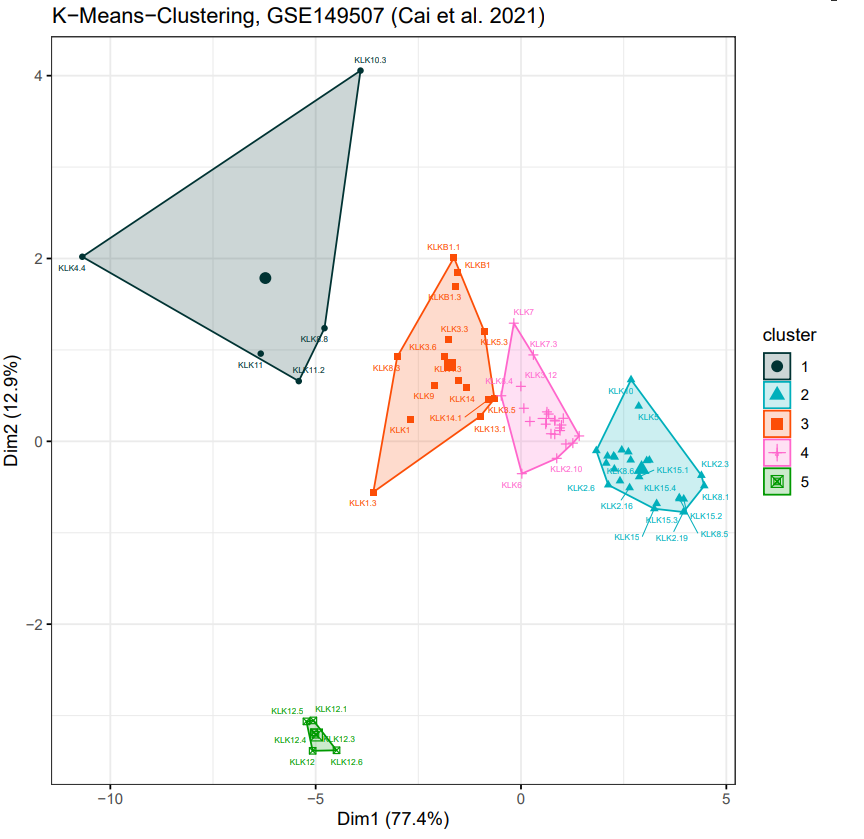
\includegraphics[width=0.5\linewidth]{images/kmeans_5_lung} 

}

\caption{K-means cluster analysis with k = 5 clusters for the lung cancer data set}\label{fig:K-means plot - lung }
\end{figure}

\hypertarget{hypothesis-testing-1}{%
\subsubsection{Hypothesis testing}\label{hypothesis-testing-1}}

The results of the PCA and the k-means indicate that for some KLKs the
expression differs between the cancerous and normal tissue. Since the
Kallikreins gene expression is not normally distributed, the Wilcoxon
signed-rank test was used. In figure X plot A, KLK4.4 was significantly
higher expressed in cancer tissue. Unlike, KLK10.3 which was
significantly higher expressed in normal tissue.

Plot B shows that KLK12 and its isoforms are significantly higher
expressed in cancer tissue. The plot also visualizes the high similarity
within isoforms, as only only identical ones were removed during the
clean up. The genes that pointed towards the normal microchips in the
PCA loadings are shown in plot C. There, KLKB1.1 and KLKB1.3 are
significantly downregulated in the cancer tissue. The only newly tested
significant gene, of those that pointed in the direction of the normal
microchips visualized in plot D, was KLK1.3. In summary five out of
seven loadings were found to have a significant expression difference
between the tissue types. Those results confirm the clear separation of
cancer and normal tissue microchips in the PCA, based on Kallikrein gene
expression.\\
In conclusion the hypothesis tests confirm the clear separation of
cancer and normal tissue microchips in the PCA based on Kallikrein
expression. Five out of seven PCA loading genes had an significant
expression difference between the tissue types.

\begin{figure}

{\centering 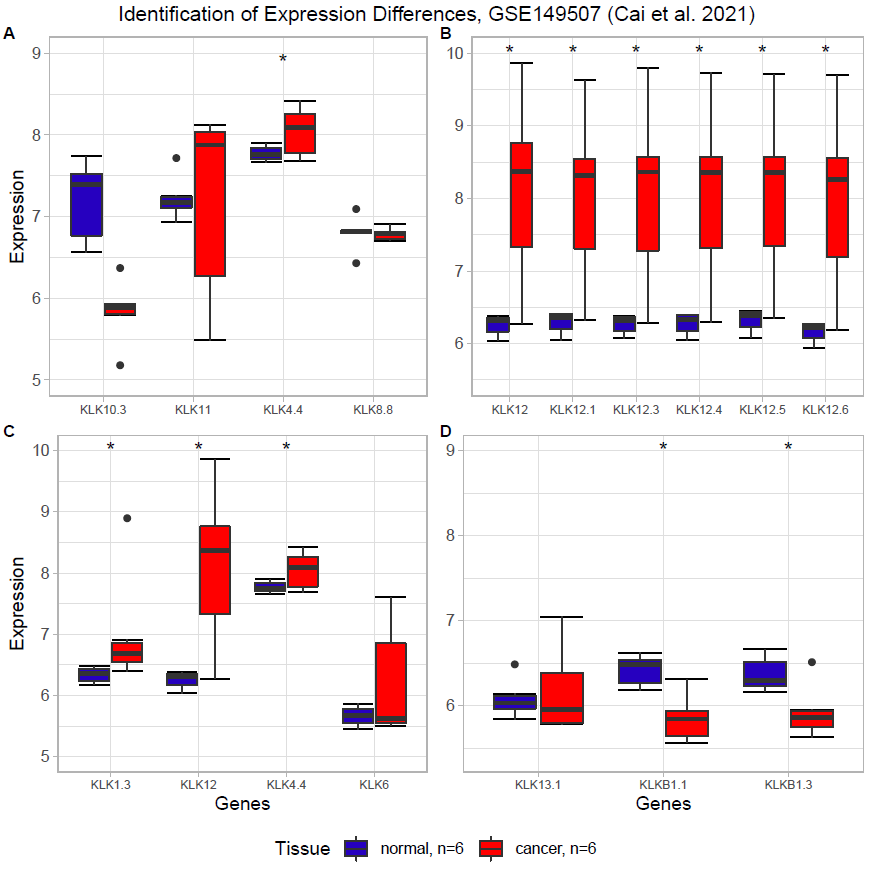
\includegraphics[width=0.5\linewidth]{images/Expr_diff_kmeans_PCA_lung} 

}

\end{figure}

\hypertarget{logistsic-regression}{%
\subsection{5. Logistsic regression}\label{logistsic-regression}}

Kallikrein mRNA or protein expression is already used in clinical
pratice as biomarkers, especially in prostate cancer (Diamandis et
al.~1998). To test whether the identified genes with a significant
expression difference were likely to predict tissue type, logistic
regression was chosen. The basic assumtions for logistsic regression
are: 1. Independency of errors, every observation has to be separate
from the others. 2. Linearity of the continuous variables in logit - the
relationship between the variable and their logit transformed outcome
should be linear. 3. Absence of multicollinearity or redundancy. 4. No
outliners with a strong influence. 5. For every independent variable
there should be at least ten outcomes (Jill C.Stoltzfus 2011).

These assumptions reveal the shortcomings of the used data and explain
the experienced problems with logistic regression. First, main
limitation of the used dataset is the low number of included microchips
(only 12, 6 from cancer and 6 from normal tissue). The number of
microchips has also been further reduced by splitting the data in a
training dataset (8 microchips) and testing dataset (4 microchips).
Therefore, expected problems of high standard errors and large
beta-coefficients for the independent variables were encountered when
including more then one independent variable. This phenomenon is also
called overfit-model. In fact, even for most individual genes, which had
been identified to have an significant expression difference, the
described problems were encountered. The only exceptions were KLK4.4 and
KLK12. Second, although genes with a correlation equal to one were
removed, some genes are still highly correlating. This is primarily true
for the different isoforms of the same gene, as visualized in figure x,
plot B (hypothesis testing KLK12 and isoforms). Therefore, the effect of
collinearity would probably cause problems, even if more microchips were
included. Hence a second cleanup, removing genes with high correlation
(e.g.~corr \textgreater{} 0.8), would probably be necessary. As
mentioned above KLK4.4 and KLK12 (and its isoforms) were the only gene
where the standard error of the independent variable was not abnormaly
high. But the p-value was, in both cases, not significant. In contrast,
the prediction of these univariant models were surprisingly accurate.
The model with KLK4.4 could predict the tissue type of 3 out of 4
microchips correctly, the model with KLK12 even predicted every tissue
type right. However, a closer look at the probabilities reveals that
these models are anything but reliable. The probabilities for normal to
be cancer tissue were mostly over a quarter, indicating a high
uncertainty.\\
In conclusion, the p-values of the independent variable in the models
were not significant, the standard errors were still large and the
predictions probabilities were not accurate. These results were not
surprising considering the low sample size.

\begin{Shaded}
\begin{Highlighting}[]
\CommentTok{#Output of the two models !}
\end{Highlighting}
\end{Shaded}

\hypertarget{discussion}{%
\subsection{Discussion}\label{discussion}}

The aim of this project was to analyse whether the expression of
Kallikrein genes in given data sets show potential biomarker
characteristics and to compare the output of statistical analysis to
already existing literature, to verify the results. Principal component
analysis with breast cancer microarray data GSE65216 (Maire et al.~2013)
provides greater insight into the expression patterns within the data
set. PCA shows that some samples are more dominated by KLK11 and KLK11.2
expression. In addition, it shows that TNBC mutations are influenced by
the expression of KLK5 and KLK6. In the heatmap four genes were
identified, which were overexpressed in at least two of the five
mutation specific microchips. KLK10.3, KLK6 for Her2, KLK11, KLK11.2 for
LumA. Those four genes are also identified as one of the twelve main
loadings of the PCA. In a previous study (Haritos et al.~2018) KLK6
expression was found to be generally downregulated in breast cancer
tissue, but in HER2 and TNBC positive tumors KLK6 was overexpressed.
Those findings are only reflected to a limited extend in this analysis.
Only Her2 was found to be significantly higher expressed than LumA. TNBC
was not significantly higher expressed compared to the other mutations.
Another study from Michaelidou et al.~reported a higher expression of
KLK8 in TNBC and Her2 positive tumors compared to LumA and LumB positive
tumors. However, this analysis could only confirm significant TNBC
overexpression for the isoform KLK8.5 compared to LumA and LumB.
Nevertheless, the boxplots of KLK8.4 and KLK8.5 show the trend of Her2
and TNBC overexpression. KLK11 shows the highest expression in breast
cancer in the research of Sano et al., 2007, thus it confirms the result
of PCA that KLK11 is upregulated. In summary, the conducted analysis
could partially conform the findings from other research groups. The
differences can probably be explained by the small amount of samples
used in this analysis. In conclusion Kallikrein gene expression can be
used for identifying tumor subtypes and even predict the outcome for a
patient (Haritos et al.~2018). Analysis of the lung cancer microarray
GSE149507 (Cai et al.~2021) demonstrated differences in the expression
of some KLKs between the cancerous and normal tissues. The result showed
that KLK4.4 was significantly higher expressed in cancer tissue. While
in normal tissue KLK10.3 expressed significantly higher. The finding of
decreased KLK11 expression in lung cancer by Sasaki et al.~could not be
confirmed. Rather, the median of cancer tissue samples is significantly
higher. Also, the conspicuity of significant high expression of KLK12
and its isoforms in cancer tissue was detected. Documented
overexpression of KLK12 could not be found in the literature, but
functional studies identified KLK12 as a pro-angiogenic factor. In
conclusion, characteristical biomarker expression has been found and
also verified by comparison with literature. High overlap of our results
with literature confirms the right usage of methods, and also indicate
that results who couldn't be verified by literature comparison, like
expression values for KLK12, could be potentially interesting to
investigate.

\hypertarget{references}{%
\subsection{References}\label{references}}

Ardlie, K.G., Deluca, D.S., Segre, A.V., Sullivan, T.J., Young, T.R.,
Gelfand, E.T., Trowbridge, C.A., Maller, J.B., Tukiainen, T., Lek, M.,
et al.~(2015). The Genotype-Tissue Expression (GTEx) pilot analysis:
Multitissue gene regulation in humans. Science 348, 648-660. Borgoño,
C.A., and Diamandis, E.P. (2004). The emerging roles of human tissue
kallikreins in cancer. Nature Reviews Cancer 4, 876-890. Cai, L., Liu,
H., Huang, F., Fujimoto, J., Girard, L., Chen, J., Li, Y., Zhang, Y.-A.,
Deb, D., Stastny, V., et al.~(2021). Cell-autonomous immune gene
expression is repressed in pulmonary neuroendocrine cells and small cell
lung cancer. Communications Biology 4.\\
Diamandis, E.P. (1998). Prostate-specific Antigen: Its Usefulness in
Clinical Medicine. Trends in Endocrinology \& Metabolism 9, 310-316.\\
Dinkelacker, M. (2007). A database of genes that are expressed in a
tissue-restricted manner to analyse promiscous gene expression in
medullary thymic epithelial cells. Diplomarbeit
(Albert-Ludwigs-Universitaet). Dinkelacker, M. (2019). Chromosomal
clustering of tissue restricted antigens. Dissertation (University
Heidelberg). Dubey, A.K., Gupta, U., and Jain, S. (2016). Analysis of
k-means clustering approach on the breast cancer Wisconsin dataset.
International Journal of Computer Assisted Radiology and Surgery 11,
2033-2047. Fischer, J., and Meyer-Hoffert, U. (2013). Regulation of
kallikrein-related peptidases in the skin -- from physiology to diseases
to therapeutic options. Thromb Haemost 110, 442-449. Haritos, C.,
Michaelidou, K., Mavridis, K., Missitzis, I., Ardavanis, A., Griniatsos,
J., and Scorilas, A. (2018). Kallikrein-related peptidase 6 (KLK6)
expression differentiates tumor subtypes and predicts clinical outcome
in breast cancer patients. Clinical and Experimental Medicine 18,
203-213. Kont, V., Laan, M., Kisand, K., Merits, A., Scott, H.S., and
Peterson, P. (2008). Modulation of Aire regulates the expression of
tissue-restricted antigens. Molecular Immunology 45, 25-33.
10.1016/j.molimm.2007.05.014. Lattin JE, S.K., Su AI, Walker JR, Zhang
J, Wiltshire T, Saijo K, Glass CK, Hume DA, Kellie S, Sweet MJ (2008).
Expression analysis of G Protein-Coupled Receptors in mouse macrophages.
Immunome Res. 4:5. Lenga Ma Bonda, W., Iochmann, S., Magnen, M., Courty,
Y., and Reverdiau, P. (2018). Kallikrein-related peptidases in lung
diseases. Biol Chem 399, 959-971. Lonsdale, J., Thomas, J., Salvatore,
M., Phillips, R., Lo, E., Shad, S., Hasz, R., Walters, G., Garcia, F.,
Young, N., et al.~(2013). The Genotype-Tissue Expression (GTEx) project.
Nature Genetics 45, 580-585. Maire, V., Némati, F., Richardson, M.,
Vincent-Salomon, A., Tesson, B., Rigaill, G., Gravier, E.,
Marty-Prouvost, B., De Koning, L., Lang, G., et al.~(2013). Polo-like
Kinase 1: A Potential Therapeutic Option in Combination with
Conventional Chemotherapy for the Management of Patients with
Triple-Negative Breast Cancer. Cancer Research 73, 813-823. Michaelidou,
K., Ardavanis, A., and Scorilas, A. (2015). Clinical relevance of the
deregulated kallikrein-related peptidase 8 mRNA expression in breast
cancer: a novel independent indicator of disease-free survival. Breast
Cancer Research and Treatment 152, 323-336. Roth, R.B., Hevezi, P., Lee,
J., Willhite, D., Lechner, S.M., Foster, A.C., and Zlotnik, A. (2006).
Gene expression analyses reveal molecular relationships among 20 regions
of the human CNS. Neurogenetics 7, 67-80. Sano, A., Sangai, T., Maeda,
H., Nakamura, M., Hasebe, T., and Ochiai, A. (2007). Kallikrein 11
expressed in human breast cancer cells releases insulin-like growth
factor through degradation of IGFBP-3. Int J Oncol 30, 1493-1498.
Sasaki, H., Kawano, O., Endo, K., Suzuki, E., Haneda, H., Yukiue, H.,
Kobayashi, Y., Yano, M., and Fujii, Y. (2006). Decreased Kallikrein 11
Messenger RNA Expression in Lung Cancer. Clinical Lung Cancer 8, 45-48.
Schmitt, M., Magdolen, V., Yang, F., Kiechle, M., Bayani, J., Yousef,
G.M., Scorilas, A., Diamandis, E.P., and Dorn, J. (2013). Emerging
clinical importance of the cancer biomarkers kallikrein-related
peptidases (KLK) in female and male reproductive organ malignancies.
Radiology and Oncology 47, 319-329. Su, A.I., Cooke, M.P., Ching, K.A.,
Hakak, Y., Walker, J.R., Wiltshire, T., Orth, A.P., Vega, R.G.,
Sapinoso, L.M., Moqrich, A., et al.~(2002). Large-scale analysis of the
human and mouse transcriptomes. Proceedings of the National Academy of
Sciences 99, 4465-4470. Su, A.I., Wiltshire, T., Batalov, S., Lapp, H.,
Ching, K.A., Block, D., Zhang, J., Soden, R., Hayakawa, M., Kreiman, G.,
et al.~(2004). A gene atlas of the mouse and human protein-encoding
transcriptomes. Proceedings of the National Academy of Sciences 101,
6062-6067. Tailor, P.D., Kodeboyina, S.K., Bai, S., Patel, N., Sharma,
S., Ratnani, A., Copland, J.A., She, J.-X., and Sharma, A. (2018).
Diagnostic and prognostic biomarker potential of kallikrein family genes
in different cancer types. Oncotarget 9, 17876-17888.
10.18632/oncotarget.24947. Uhlen, M., Fagerberg, L., Hallstrom, B.M.,
Lindskog, C., Oksvold, P., Mardinoglu, A., Sivertsson, A., Kampf, C.,
Sjostedt, E., Asplund, A., et al.~(2015). Tissue-based map of the human
proteome. Science 347, 1260419-1260419. Yousef, G.M., Chang, A.,
Scorilas, A., and Diamandis, E.P. (2000). Genomic Organization of the
Human Kallikrein Gene Family on Chromosome 19q13.3--q13.4. Biochemical
and Biophysical Research Communications 276, 125-133.
10.1006/bbrc.2000.3448. Yousef, G.M., Magklara, A., and Diamandis, E.P.
(2000). KLK12 Is a Novel Serine Protease and a New Member of the Human
Kallikrein Gene Family---Differential Expression in Breast Cancer.
Genomics 69, 331-341. Yousef, G.M., Yacoub, G.M., Polymeris, M.E.,
Popalis, C., Soosaipillai, A., and Diamandis, E.P. (2004). Kallikrein
gene downregulation in breast cancer. British Journal of Cancer 90,
167-172. Zhang, Y., Bhat, I., Zeng, M., Jayal, G., Wazer, D.E., Band,
H., and Band, V. (2006). Human kallikrein 10, a predictive marker for
breast cancer. 387, 715-721.

\end{document}
